\section{Results}
In this section we report statistics and resource utilization of our design, and analyze the resulting wave forms.
\subsection{Sequential Implementation}
\subsubsection{Resources}
The synthesis report gives us the following properties:
\begin{verbatim}
# Multipliers                                          : 1
 16x16-bit multiplier                                  : 1
# Adders/Subtractors                                   : 1
 32-bit adder                                          : 1
# Counters                                             : 1
 6-bit up counter                                      : 1
# Registers                                            : 594
 Flip-Flops                                            : 594
\end{verbatim}
As intended our filter only uses one multiplier. The 32 bit adder is used in the FIR multiply accumulate, the 6 bit counter is used to indicate which state the filter is in. The number of registers is roughly the sum of the number of data\_in registers ($32 \cdot 16 = 512$), plus $2 \cdot 32$ for the multiply and accumulate registers, which adds up to 576. The rest is explained by some req, ack buffers etc. 
\subsubsection{Properties}
The sample frequency of the filter is as follows:
\begin{itemize}
\item
Synthesis report
\begin{itemize}
\item Minimum period: 7.351ns
\item Maximum Frequency: 136.037MHz
\end{itemize}
\item
Post-PAR static timing report
\begin{itemize}
\item  Minimum period:   9.137ns  
\item Maximum frequency: 109.445MHz
\end{itemize}
\end{itemize}
The sample frequency is lower in the static timing report, because it takes into account how the circuit will actually be laid out on the FPGA. The important thing here is that the sample frequency meets the 100 MHz requirement, which means this filter is fast enough to process the audio file using only one multiplier.
\subsection{Strength Reduced}
\subsubsection{Resources}
todo
\subsubsection{Properties}
todo
\subsection{Analysis of filter output}
Here we will analyze the effect of the filter on the input signal. This section corresponds to both the sequential and the strength reduced filter, since they implement the same function, a low pass FIR filter.\\
The effect of the filter is clearly shown in figure  ~\ref{fig:diff}, where the original signal is plotted together with the filtered signal and the difference between the two signals. It is clear to see that the high frequency harmonics in the original signal have been removed in the filtered signal, because it is much smoother. This is also demonstrated by in the difference signal, which only shows high harmonics. To calculate the difference, we used a scaling factor because the filtered signal is weaker than the original signal. This is caused by the filter coefficients which are:
\begin{gather*}
14,15,16,17,17,16,15,14
\end{gather*}
The sum of these coefficients is $124$, which gives us a scaling factor of $\frac{256}{124}$. We also shifted the filtered signal by 4, half of the number of coefficients, to have the signals line up better. The figure also shows the start up noise of the filter; the first 32 values are incorrect.

\begin{figure}
\begin{center}
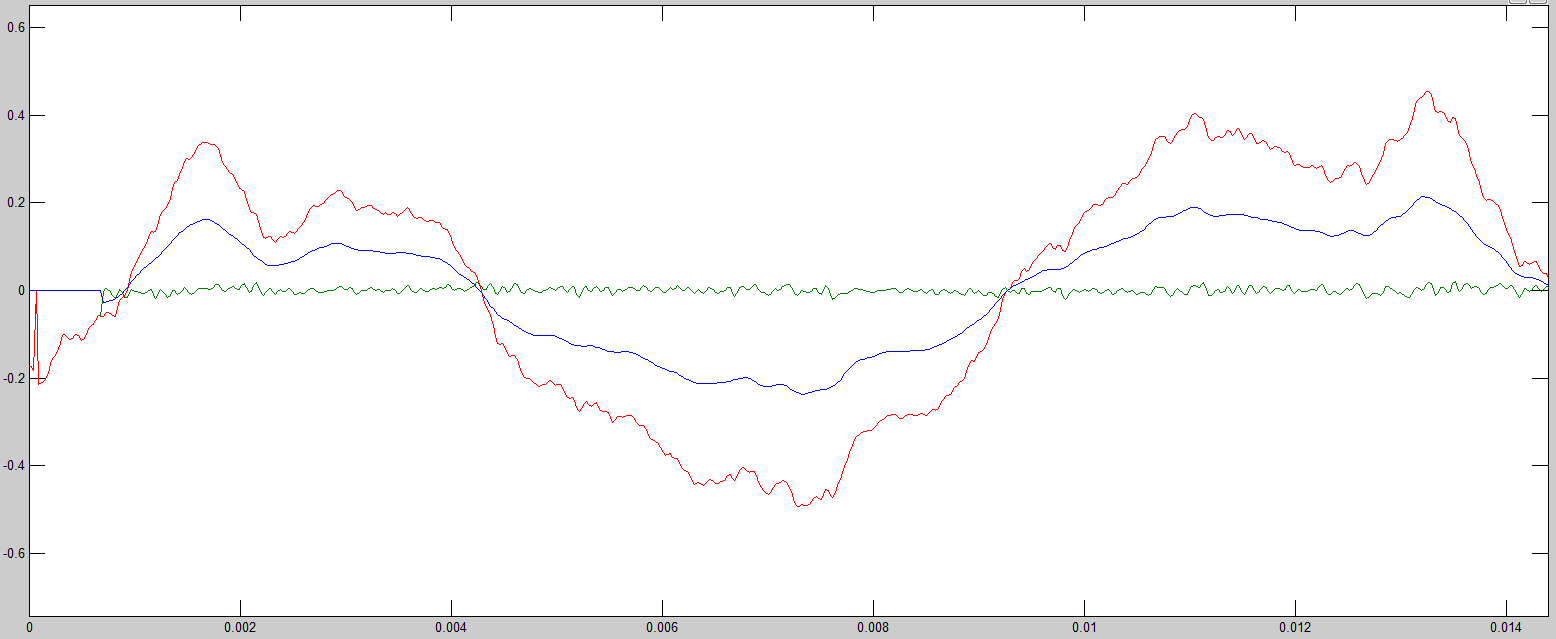
\includegraphics[width=0.7\textwidth]{images/diff.png}
\caption{Part the original signal (red), the filtered signal (blue), and the signal \mbox{(original - $\frac{256}{124}$ * filtered signal)} (green).}
\label{fig:diff}
\end{center}
\end{figure}

Another visualization of the effect of the filter is shown in figure  ~\ref{fig:spectrum} in which the signals are plotted in the frequency domain. The high frequency harmonics are clearly missing in the filtered signal, the stop frequency is around 4000 Hz. 

\begin{figure}
\begin{center}
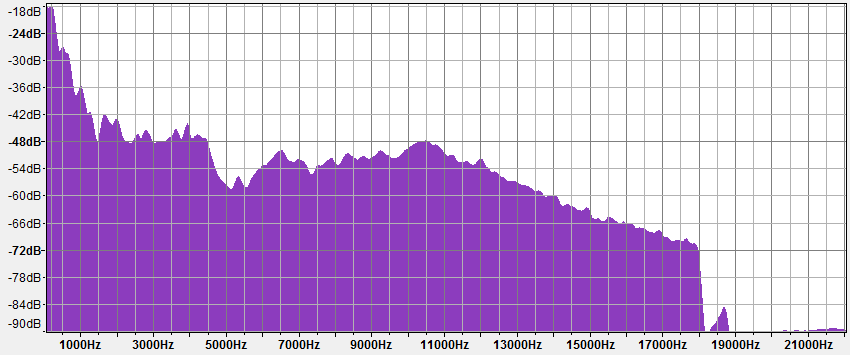
\includegraphics[width=0.7\textwidth]{images/spectrum_input.png}
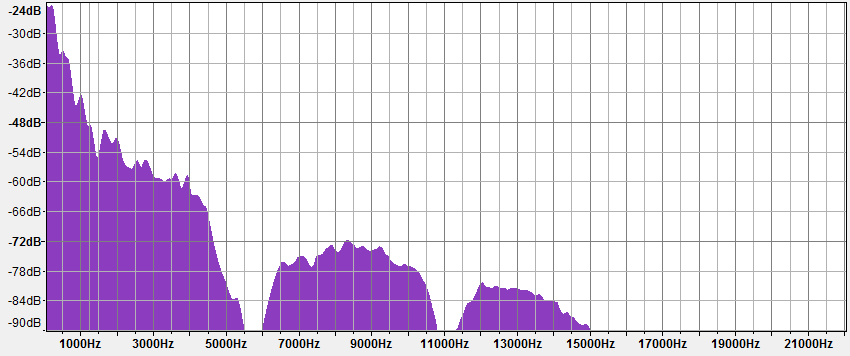
\includegraphics[width=0.7\textwidth]{images/spectrum_output.png}
\caption{Plot in the frequency domain of the original signal (top) and the signal after filtering (bottom).}
\label{fig:spectrum}
\end{center}
\end{figure}


\FloatBarrier
